\documentclass[a4paper,12pt]{article} % добавить leqno в [] для нумерации слева
\usepackage[a4paper,top=1.3cm,bottom=2cm,left=1.5cm,right=1.5cm,marginparwidth=0.75cm]{geometry}
%%% Работа с русским языком
\usepackage{cmap}					% поиск в PDF
\usepackage{mathtext} 				% русские буквы в фомулах
\usepackage[T2A]{fontenc}			% кодировка
\usepackage[utf8]{inputenc}			% кодировка исходного текста
\usepackage[english,russian]{babel}	% локализация и переносы

\usepackage{graphicx}

\usepackage{wrapfig}
\usepackage{tabularx}

\usepackage{hyperref}
\usepackage[rgb]{xcolor}
\hypersetup{
colorlinks=true,urlcolor=blue
}
\usepackage{multirow}
\usepackage{hhline}


%%% Дополнительная работа с математикой
\usepackage{amsmath,amsfonts,amssymb,amsthm,mathtools} % AMS
\usepackage{icomma} % "Умная" запятая: $0,2$ --- число, $0, 2$ --- перечисление

%% Номера формул
\mathtoolsset{showonlyrefs=true} % Показывать номера только у тех формул, на которые есть \eqref{} в тексте.

%% Шрифты
\usepackage{euscript}	 % Шрифт Евклид
\usepackage{mathrsfs} % Красивый матшрифт

%% Свои команды
\DeclareMathOperator{\sgn}{\mathop{sgn}}

%% Перенос знаков в формулах (по Львовскому)
\newcommand*{\hm}[1]{#1\nobreak\discretionary{}
{\hbox{$\mathsurround=0pt #1$}}{}}

\begin{document}
	
	\begin{titlepage}
	\begin{center}
		{\large МОСКОВСКИЙ ФИЗИКО-ТЕХНИЧЕСКИЙ ИНСТИТУТ (НАЦИОНАЛЬНЫЙ ИССЛЕДОВАТЕЛЬСКИЙ УНИВЕРСИТЕТ)}
	\end{center}
	\begin{center}
		{\large Физтех-школа электроники, фотоники и молекулярной физики}
	\end{center}
	
	
	\vspace{4.5cm}
	{\huge
		\begin{center}
			{Лабораторная работа 4.4.1}\\
			Амплитудная дифракционная решетка
		\end{center}
	}
	\vspace{2cm}
	\begin{flushright}
		{\LARGE Салтыкова Дарья \\
			\vspace{0.5cm}
			Б04-105}
	\end{flushright}
	\vspace{8cm}
	\begin{center}
		Долгопрудный 2023
	\end{center}
\end{titlepage}

\section{Введение}

\noindent
\textbf{Цель работы:} знакомство с работой и настройкой гониометра Г5, определение спектральных характеристик амплитудной решетки.
\medskip

\noindent \textbf{В работе используются:} гониометр, дифракционная решетка, ртутная лампа.

\medskip

\section{Теоретические сведения}

\noindent Основное соотношение приближенной теории дифракционной решётки:
	\begin{equation}
	d\sin \varphi_m = m\lambda.
	\end{equation}
	Угловая дисперсия $D$ характеризует угловое расстояние между близкими спектральными линиями:
	\begin{equation}
	D = \frac{d\varphi}{d\lambda} = \frac{m}{d \cos \varphi}=\frac{m}{\sqrt{d^{2}-m^{2} \lambda^{2}}}.
	\end{equation}


\section{Экспериментальная установка}

\noindent При работе с дифракционной решёткой основной задачей является точное измерение углов, при которых наблюдаются главные максимумы для различных длин волн. В нашей работе для измерения углов используется гониометр Г5. Принципиальная схема экспериментальной установки приведена на рисунке.

\begin{center}

	\begin{figure}[h!]
		
		\label{inst}
		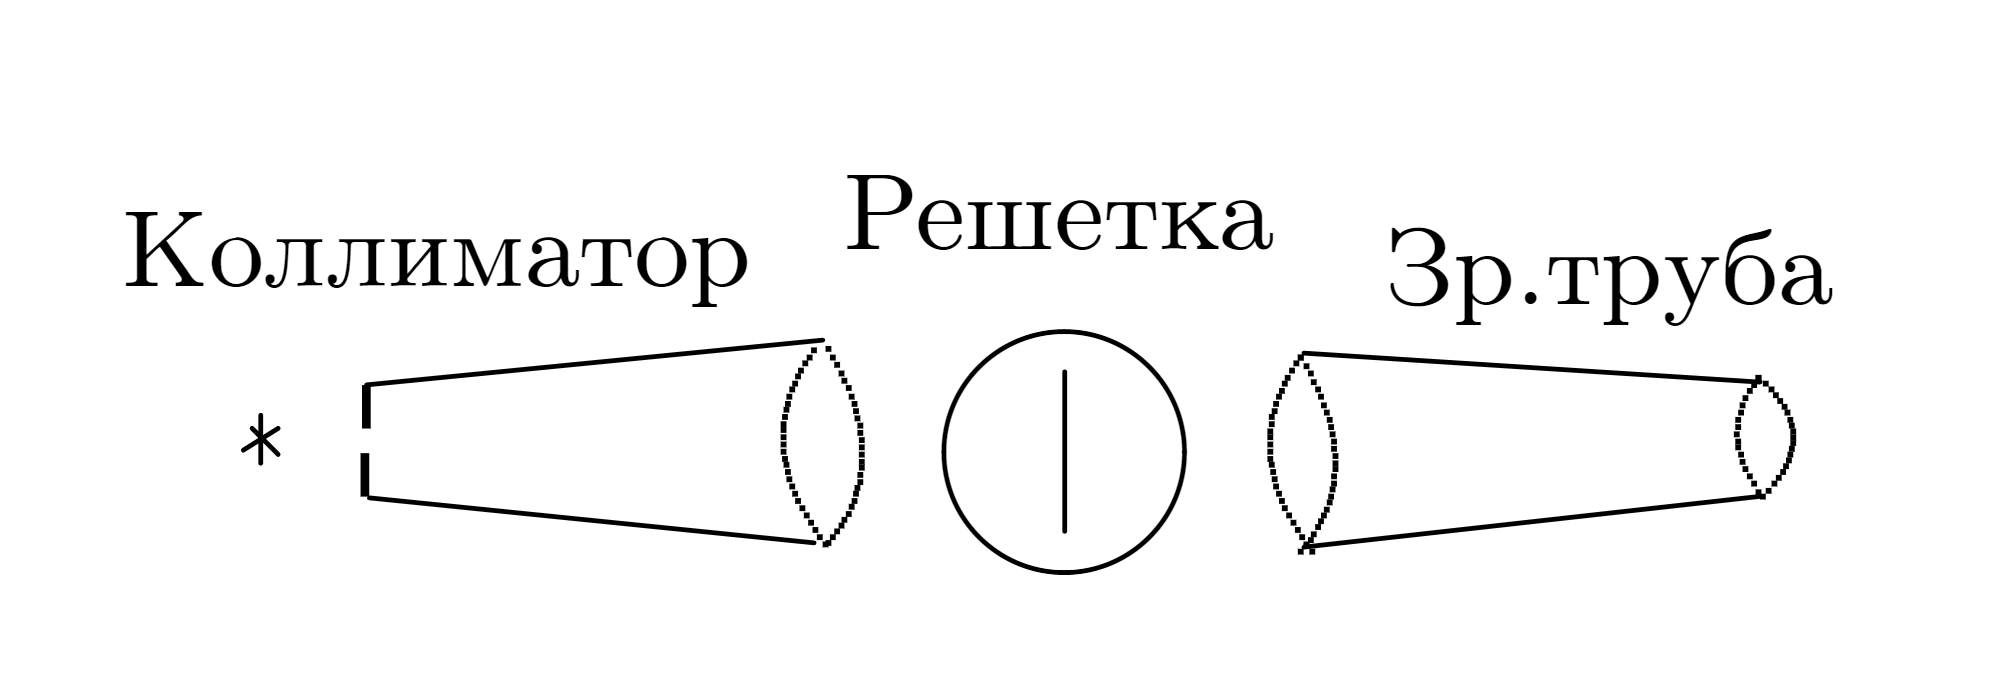
\includegraphics[scale=0.2]{inst.png}
	\end{figure}
	
\end{center}


\section{Ход работы}

\noindent 1. Измерим угловые координаты спектральных линий ртути в $ \pm1 $ порядках, рассчитаем углы дифракции $\varphi_m$. См. таблицу в Приложении.

\medskip

\noindent 2. Измерим угловые координаты линий жёлтого дублета для $\pm1$ порядка. Для оценки разрешающей способности спектрального прибора измерим угловую ширину одной из линий жёлтого дублета по нулям интенсивности в $\pm1$ порядках.

\begin{table}[h!]
\begin{tabular}{|l|l|l|}
\hline
m  & Ширина & $\delta \varphi$ \\ \hline
1  & 37''   & 3' 40''       \\ \hline
-1 & 57''   & 3' 24''       \\ \hline
\end{tabular}
\end{table}

\medskip

\noindent 3. Построим график зависимости $sin\varphi_m$ от длины волны.

\begin{table}[]
\begin{tabular}{ll}
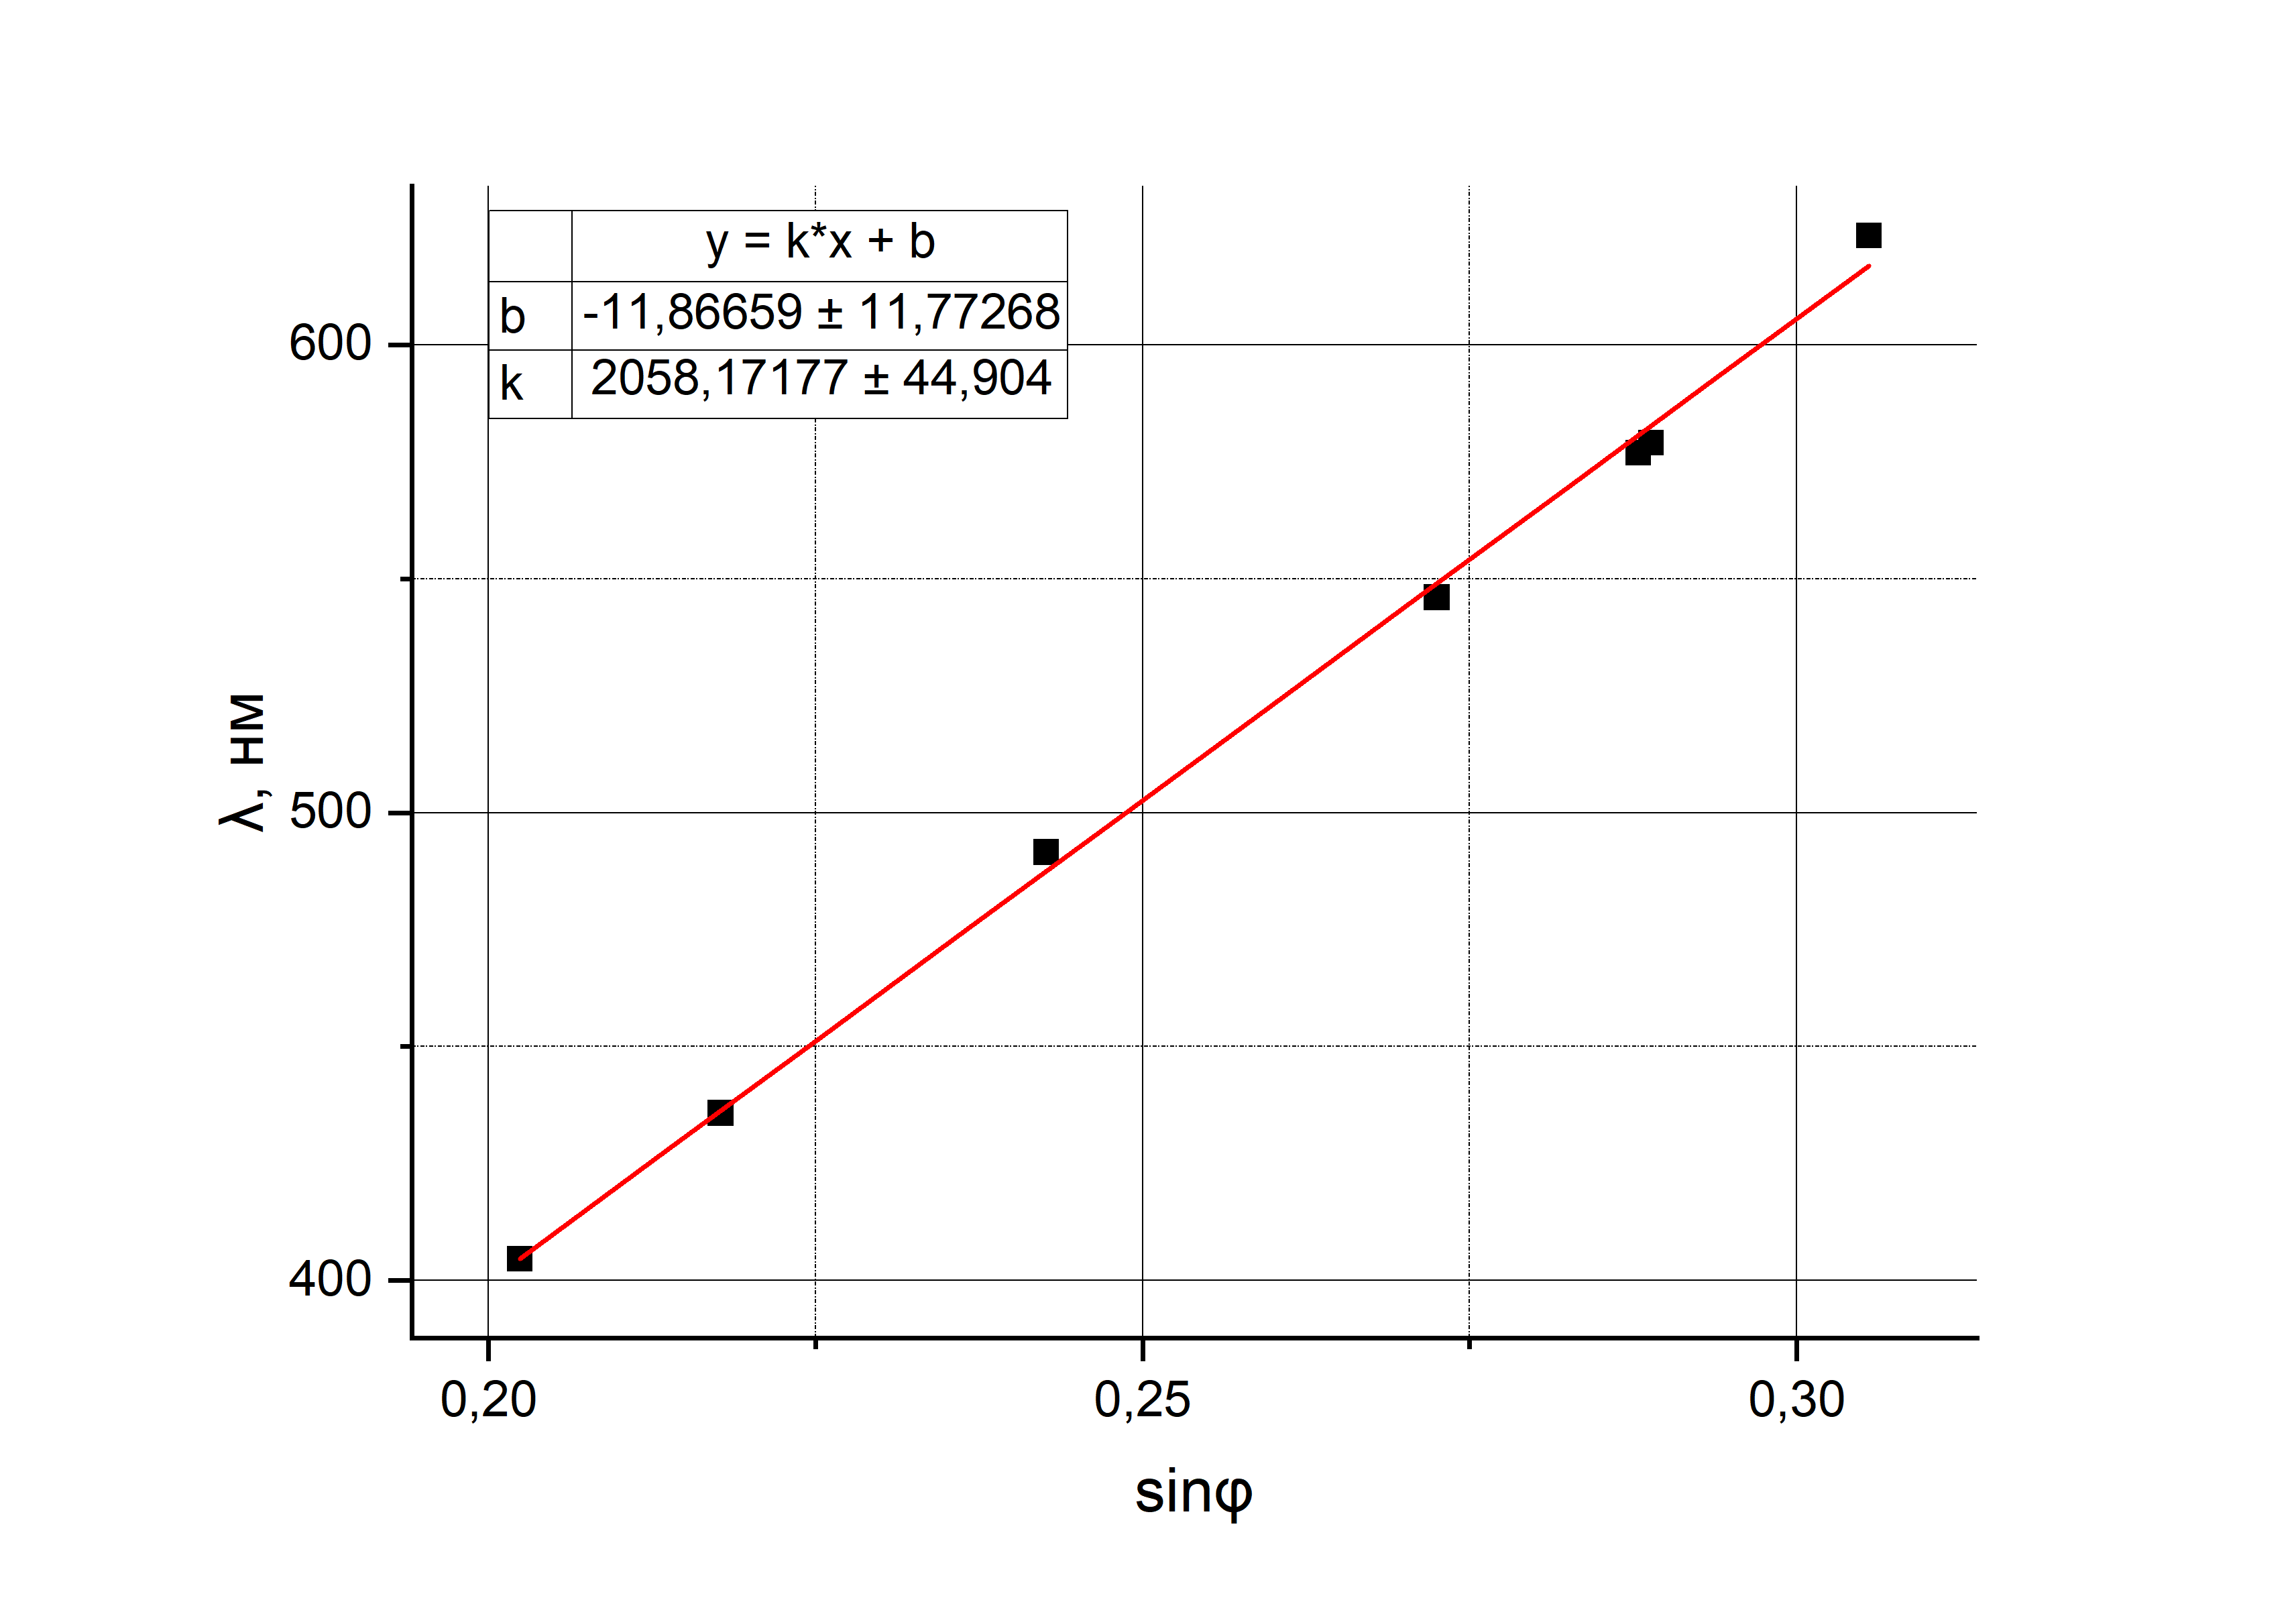
\includegraphics[width=0.5\linewidth]{gr1.png} & 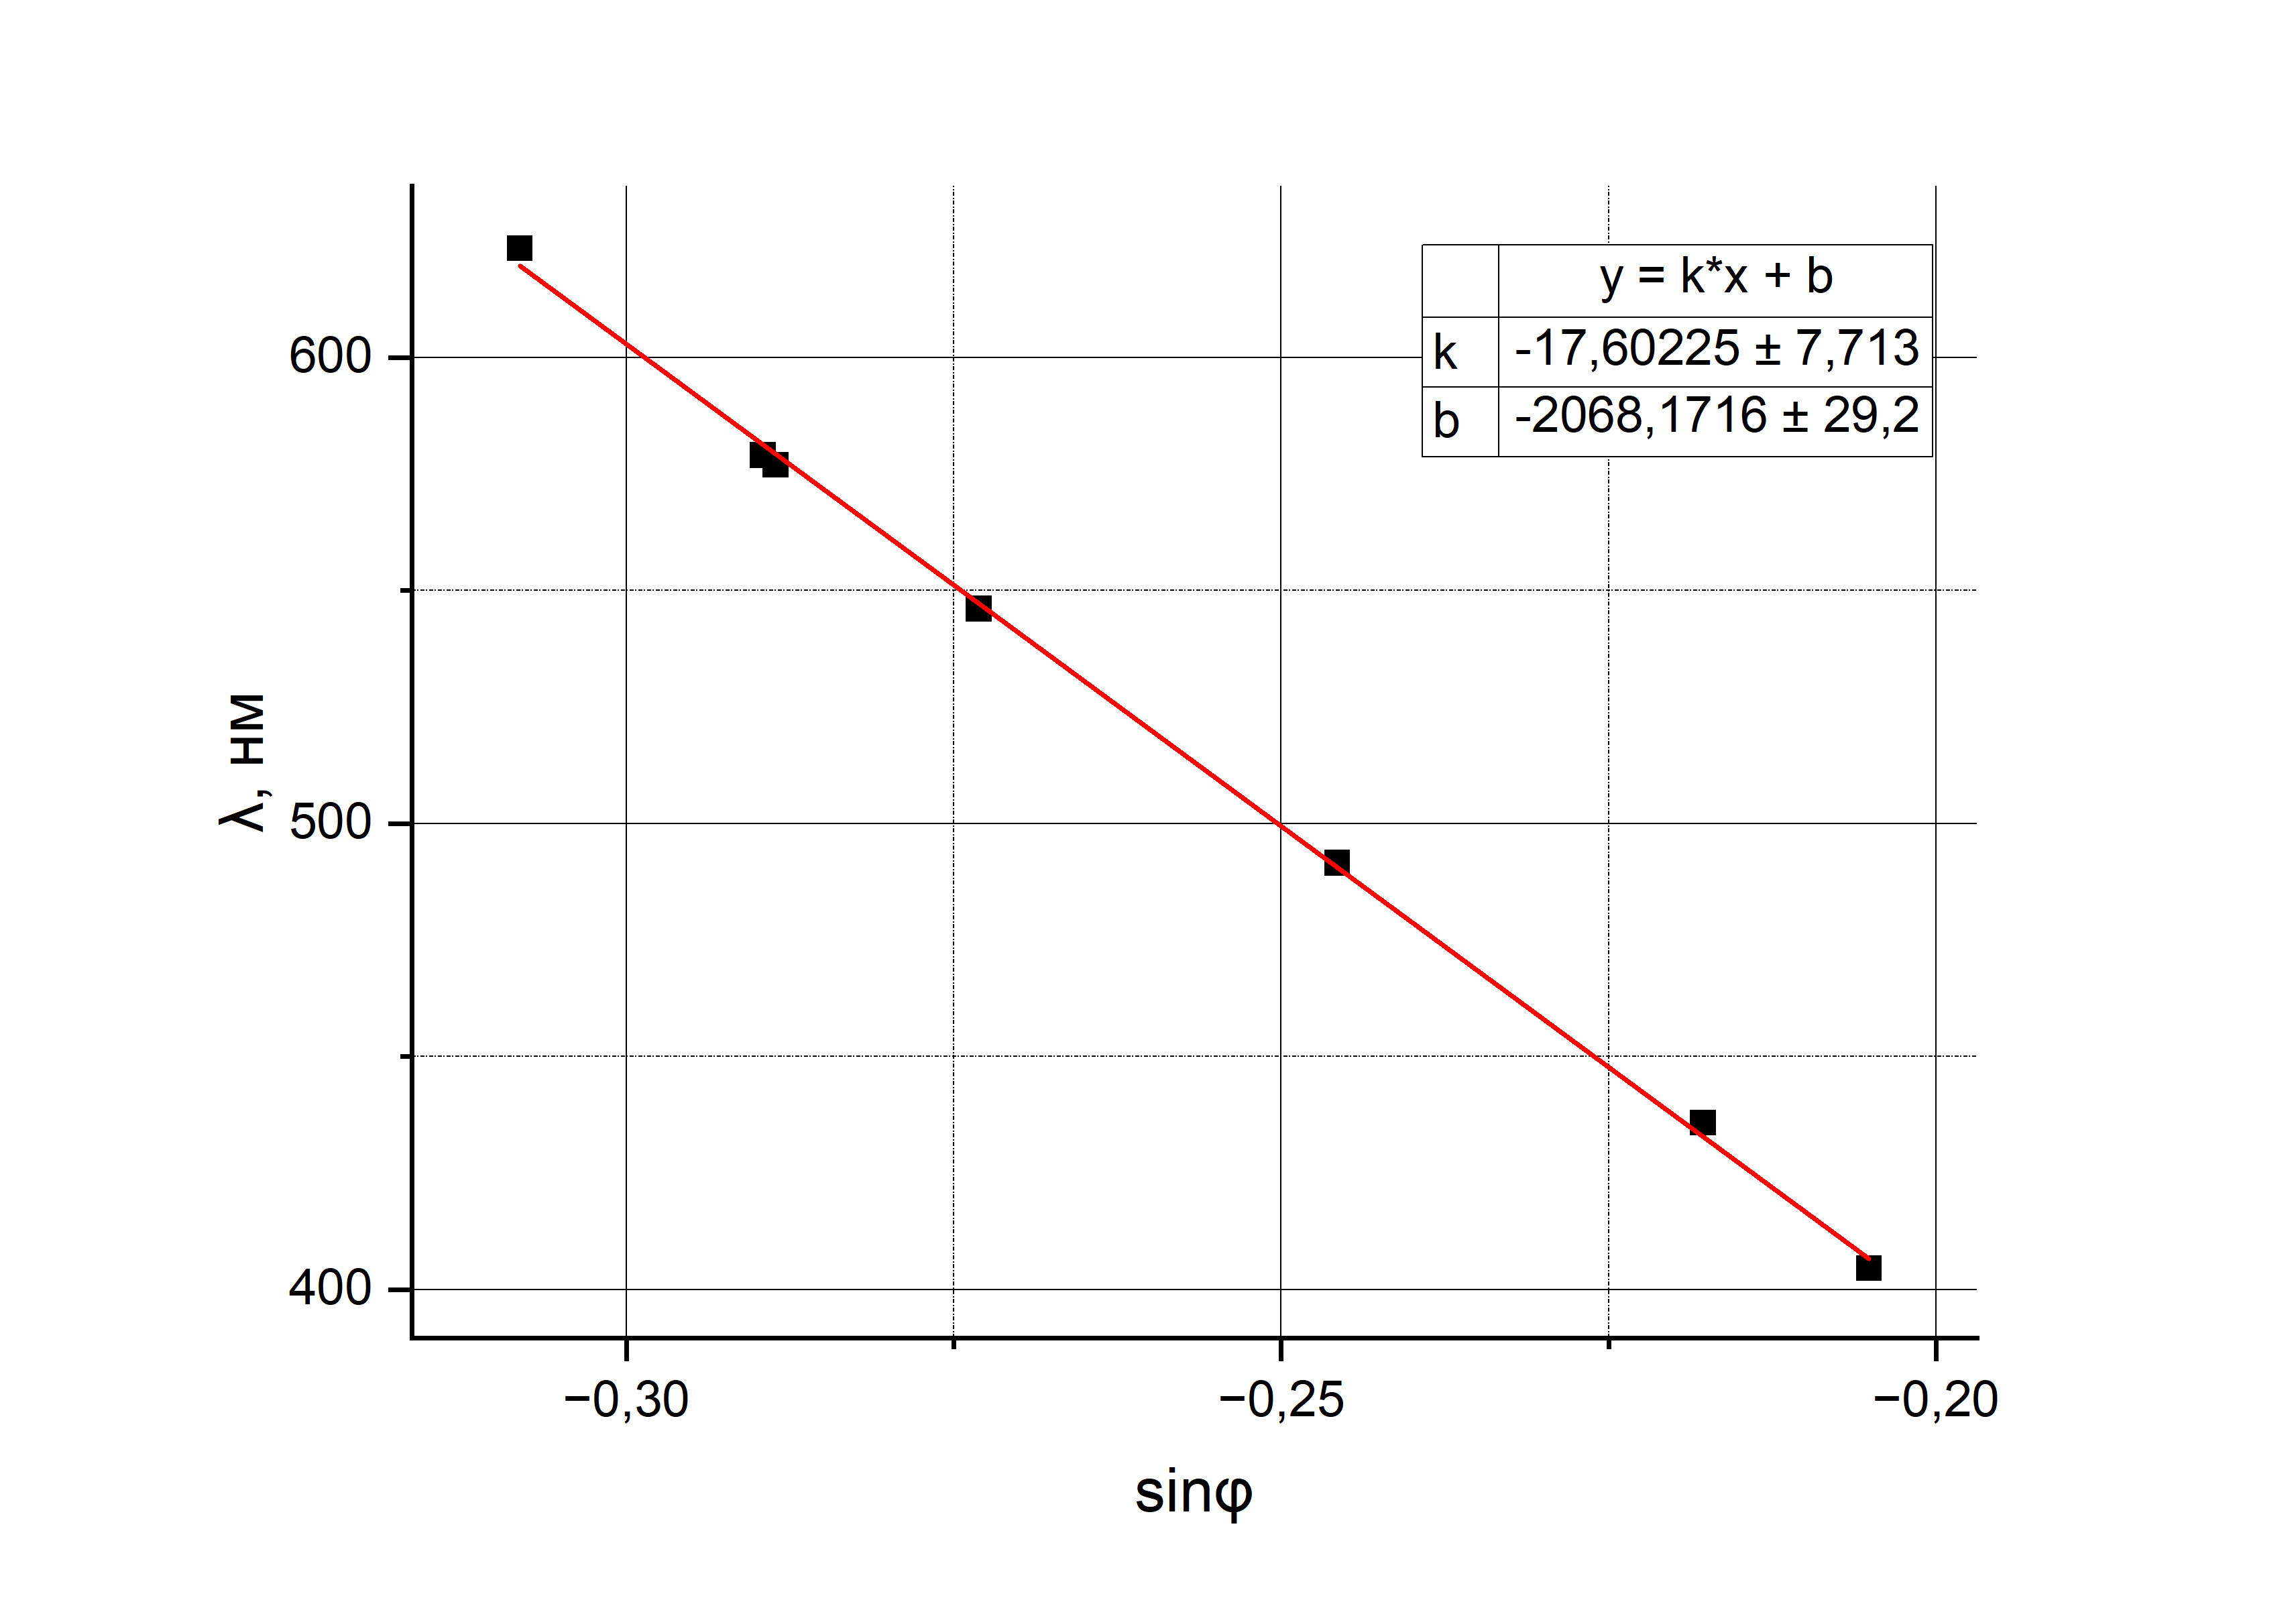
\includegraphics[width=0.5\linewidth]{gr2.png} \\
\multicolumn{1}{c}{m = 1}                        & \multicolumn{1}{c}{m = -1}                      
\end{tabular}
\end{table}

\medskip

\noindent Из графиков $d = (2063 \pm 15)\text{ мм}$.

\medskip

\noindent 4. Рассчитаем по линиям жёлтого дублета угловую дисперсию в спектрах
разного порядка.

\begin{table}[h!]
\begin{tabular}{|l|l|l|l|}
\hline
m  & $\delta \phi$ & $D_\text{эксп}, 10^{-5}   \frac{\text{рад}}{\buildrel _{\circ} \over {\mathrm{A}}}$ & $D_\text{теор}, 10^{-5}   \frac{\text{рад}}{\buildrel _{\circ} \over {\mathrm{A}}}$ \\ \hline
1  & 3' 40''       & 5,08 $\pm 0,15$                      & 5,062                                             \\ \hline
-1 & 3' 24''       & 4,70 $\pm 0,14$                      & 5,062                                             \\ \hline
\end{tabular}
\end{table}

\noindent 5. Оценим разрешимый спектральный интервал: 
\begin{equation}
			\delta\lambda \approx \Delta\varphi/D = (2,73 \pm 0,11) \buildrel _{\circ} \over {\mathrm{A}};
		\end{equation}


\noindent разрешающую способность:

 \begin{equation}
			R \approx \frac{\lambda}{\delta\lambda} = 2117 \pm 85;
		\end{equation}

\noindent число эффективно работающих штрихов решётки: 

\begin{equation}
			N \approx R/m = 2885;
		\end{equation}

\noindent эффективный размер:
		
		\begin{equation}
			L \approx Nd = 4,4\; \text{мм.}
		\end{equation}


\section{Вывод}

\medskip

\noindent В ходе работы были исследованы спектральные линии ртути, определен шаг решётки, её угловая дисперсия, а также её эффективный размер. Полученные результаты близки к теоретическим вычислениям.

\newpage

\section{Приложение}

\begin{table}[h!]
\begin{tabular}{|c|l|l|l|l|}
\hline
\multicolumn{1}{|l|}{$\text{порядок}$} & $\text{цвет}$       & $\varphi$               & $\lambda, \text{ нм}$ & $sin\varphi$ \\ \hline
\multirow{7}{*}{1}                     & $\text{фиолетовый}$ & $168^\circ 19' 27''$ & 404,66                & 0,202374  \\ \cline{2-5} 
                                       & $\text{синий}$      & $167^\circ 25' 25''$ & 435,83                & 0,217741  \\ \cline{2-5} 
                                       & $\text{голубой}$    & $165^\circ 57' 31''$ & 491,60                & 0,242623  \\ \cline{2-5} 
                                       & $\text{зеленый}$    & $164^\circ 11' 17''$ & 546,07                & 0,272481  \\ \cline{2-5} 
                                       & $\text{желтый 1}$   & $163^\circ 16' 10''$ & 576,96                & 0,287871  \\ \cline{2-5} 
                                       & $\text{желтый 2}$   & $163^\circ 12' 38''$ & 579,07                & 0,288855  \\ \cline{2-5} 
                                       & $\text{красный}$    & $162^\circ 12' 38''$ & 623,40                & 0,305520  \\ \hline
\multirow{7}{*}{-1}                    & $\text{фиолетовый}$ & $191^\circ 50' 13''$ & 404,66                & -0,20513  \\ \cline{2-5} 
                                       & $\text{синий}$      & $192^\circ 34' 49''$ & 435,83                & -0,21781  \\ \cline{2-5} 
                                       & $\text{голубой}$    & $194^\circ 13' 30''$ & 491,60                & -0,24573  \\ \cline{2-5} 
                                       & $\text{зеленый}$    & $195^\circ 50' 53''$ & 546,07                & -0,27309  \\ \cline{2-5} 
                                       & $\text{желтый 1}$   & $196^\circ 46' 30''$ & 576,96                & -0,28861  \\ \cline{2-5} 
                                       & $\text{желтый 2}$   & $196^\circ 49' 59''$ & 579,07                & -0,28958  \\ \cline{2-5} 
                                       & $\text{красный}$    & $197^\circ 56' 50''$ & 623,40                & -0,308141 \\ \hline
\end{tabular}
\end{table}


\end{document}